\section{\AP{}Semantic Path-Width}
\label{sec:semantic-path-width}
% \diego{``Deciding Boundedness'' n'est pas ce qu'on fait...}

In this section, we extend our results to "path-width". Our motivation lies in the fact that "UC2RPQs" of bounded "semantic path-width" admit a "paraNL"\footnote{This is the parametrized counterpart of non-deterministic logspace.} algorithm for the 
"evaluation problem"---see \Cref{thm:evaluation-bounded-pathwidth}---to be compared with "FPT" for bounded "semantic tree-width".

\subsection{\AP{}Path-Width of Queries}

Recall that for tree-width, for any $k \geq 2$, we proved that a "CRPQ" is equivalent to a
finite union of "C2RPQs" of "tree-width" at most $k$ "iff" it is equivalent to finite union of
"CRPQs" of "tree-width" at most $k$ (\Cref{thm:closure-under-sublanguages}). In other words, "two-way navigation" does not help to minimize further the "semantic tree-width" of a query that does not use "two-way navigation". This property does not hold for $k=1$
(\Cref{rk:closure-under-sublanguages-k1}). We show in \Cref{rk:path-width:oneway-vs-twoway} that it also does not hold for
"path-width", no matter the value of $k \geq 1$.

This motivates the following two definitions:
\begin{itemize}
	\itemAP the ""semantic path-width"" of a "UC2RPQ" is the minimal "path-width"
	of a "UC2RPQ" equivalent to it
	\itemAP the ""one-way semantic path-width"" of a "UCRPQ" is the minimal "path-width"
		of a "UCRPQ" equivalent to it.
\end{itemize}
For a given "UCRPQ", the two natural numbers are well-defined, and the former is always less or equal to
the letter.
The \AP ""semantic path-width $k$ problems"" ask, given a "UCRPQ" (resp.\ "UC2RPQ"), if it has
"semantic path-width" (resp.\ "one-way semantic path-width") at most $k$.

In this section, we first show that the "semantic path-width $k$ problems"
are decidable (\Cref{thm:decidability-sempw}), and then 
after showing that evaluation of "UC2RPQs" of bounded "path-width" is "NL" (\Cref{lemma:evaluation-bounded-pathwidth}) we deduce that for the "evaluation problem" for
"UC2RPQs" of bounded "semantic path-width" (in particular, this captures the
case of "UCRPQs" of bounded "one-way semantic path-width") is in
"para-NL" when parametrized in the size of the query (\Cref{thm:evaluation-bounded-pathwidth}).

\subsection{\AP{}Deciding Bounded Semantic Path-Width}

The key (implicit) ingredient in the proof of \Cref{thm:closure-under-sublanguages,cor:mua-exists-effective} is that "tree-width" at most $k$ is closed under "expansions" (\Cref{fact:refinement-tw}). Unfortunately, this property fails for "path-width".

\begin{figure}[tbp]
	\centering
	\subfloat[Graph $\+G_k$ with a "path decomposition" of "width" $k$, with three "bags".]{%
		\AP\label{subfig:pw-not-closed-original}%
		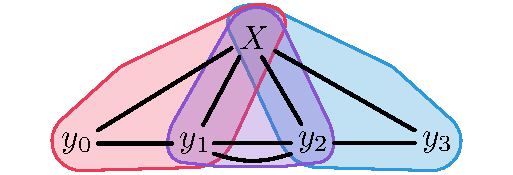
\includegraphics[width=.38\textwidth]{pw-not-closed-original}
	}
	\hspace{1.5em}
	\subfloat["Expansion" $\+G'_k$ of $\+G_k$ with a "path decomposition" of "width" $k+1$, with three "bags".]{%
		\AP\label{subfig:pw-not-closed-path-dec-horizontal}%
		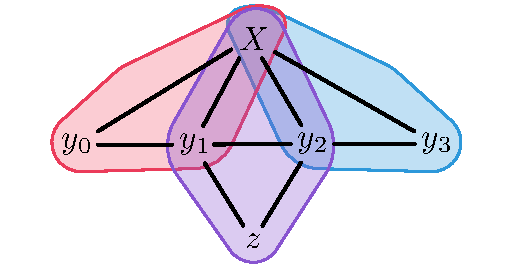
\includegraphics[width=.38\textwidth]{pw-not-closed-path-dec-horizontal}
	}
	\bigskip
	\subfloat["Tree decomposition" of $\+G'_k$ of "width" $k$, with four "bags".]{%
		\AP\label{subfig:pw-not-closed-tree-dec}	
		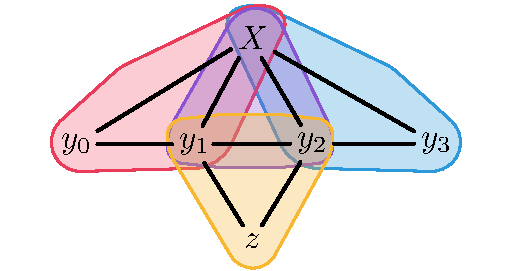
\includegraphics[width=.38\textwidth]{pw-not-closed-tree-dec}
	}
	\hspace{1.5em}
	\subfloat["Path decomposition" of $\+G'_k$ of "width" $k+1$, with three "bags".]{%
		\AP\label{subfig:pw-not-closed-path-dec-vertical}
		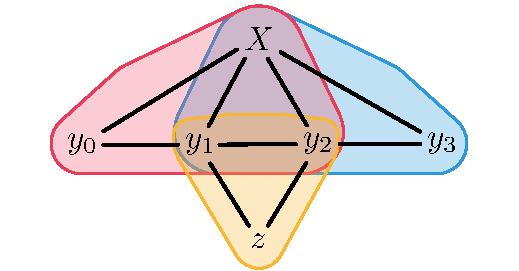
\includegraphics[width=.38\textwidth]{pw-not-closed-path-dec-vertical}
	}
	\caption{
		\AP\label{fig:pw-not-closed}
		The class of multigraphs with "path-width" at most $k \geq 1$ is not closed under "expansions":
		illustration of a multigraph $\+G_k$ of "path-width" $k$ (\Cref{subfig:pw-not-closed-original})
		whose "expansion" $\+G'_k$ has "path-width" $k+1$ (\Cref{subfig:pw-not-closed-path-dec-horizontal,subfig:pw-not-closed-path-dec-vertical})---but
		"tree-width" $k$ (\Cref{subfig:pw-not-closed-tree-dec}). Set $X$ represents a $(k-1)$-clique.
	}
\end{figure}
\begin{restatable}{fact}{pathwidthnotclosed}
	\AP\label{fact:pw-not-closed}
	For each $k \geq 1$, the class of graphs of "path-width" at most $k$ is not
	closed under "expansions".
\end{restatable}

The counterexample is illustrated in \Cref{fig:pw-not-closed}. A formal proof can be found
in \Cref{apdx-sec:path-width-not-closed-refinements}.
\begin{restatable}{rem}{onewayVsTwowayPw}
	\AP\label{rk:path-width:oneway-vs-twoway}
	Contrary to the case of "semantic tree-width", for every $k$ there are "CRPQs" which are of "semantic path-width" $k$ but not of "one-way semantic path-width" $k$.
\end{restatable}
\begin{proof}
	Indeed, let
	\begin{align*}
		\gamma_k(\bar x, \bar y) \defeq\hspace{1em}
		\bigl( & \bigwedge_{1 \leq i < j \leq k-1} x_i \atom{a} x_j \bigr)
		\;\land\; \bigl(\bigwedge_{1 \leq i \leq k-1} \bigwedge_{0 \leq j \leq 3} x_i \atom{b} y_i \bigr) \\
		\land\; \bigl( & \bigwedge_{0 \leq j < 3} y_i \atom{c} y_{i+1}\bigr)
		\;\land\; y_1 \atom{d} z \;\land\; y_2 \atom{e} z,
	\end{align*}
	whose underlying graph corresponds to \Cref{subfig:pw-not-closed-path-dec-horizontal}.
	Observe that it is a "core" and that only $z$ is existentially quantified.
	Then in $\gamma_k(\bar x, \bar y)$, one can replace the two "atoms"
	$y_1 \atom{d} z \;\land\; y_2 \atom{e} z$ by $y_1 \atom{d\, e^{-}} y_2$, while preserving the semantics. The underlying graph of this new query being \Cref{subfig:pw-not-closed-original}, it shows that $\gamma_k$ has "semantic path-width" $k$.

	Finally, we claim that $\gamma_k$ has "one-way semantic path-width" $k+1$.
	The upper bound follows from \Cref{subfig:pw-not-closed-path-dec-vertical}.
	For the lower bound, consider a "UCRPQ" $\Delta_k(\bar x, \bar y)$ such that
	$\gamma_k \semequiv \Delta_k$. Since $\gamma_k$ is a "CQ", the "equivalence" implies
	that there exists an "expansion" $\xi$ of a "CRPQ" of $\Delta_k$ such $\gamma_k$ and
	$\xi$ are homomorphically equivalent. Since $\gamma_k$ is a "core", it follows that
	$\xi$ contains it as a subgraph. Hence, the underlying directed multigraph
	of the "CRPQ" in $\Delta_k$ from which $\xi$ originated
	must contain a "one-way contraction" of $\xi$ as a subgraph.
	But the only "one-way contraction" of $\xi$ is itself, and so it follows that
	at least one "CRPQ" in $\Delta_k$ contains the underlying graph of $\xi$ as a subgraph.
	Therefore, $\Delta_k$ has "path-width" at least $k+1$, which concludes the proof
	that the "one-way semantic path-width" of $\gamma_k$ is at least (and hence exactly) $k+1$.
\end{proof}

As done for "contracted tree-width", we define "contracted path-width".
\begin{definition}
	\AP
	Define the ""contracted path-width"" (resp.\ ""one-way contracted path-width"")
	of a "C2RPQ" as the minimum of the "path-width" among its "contractions" (resp.\ of its "one-way contractions"). Let $\intro*\ContrPw$ and $\intro*\ContrPwOneWay$ be, respectively, the set of all "C2RPQs" of "contracted path-width" at most $k$ and of "CRPQs" of "one-way contracted path-width" at most $k$.
\end{definition}
The statements and proofs of this section are analogous to the ones of \Cref{sec:acyclic-queries} in the context of "contracted tree-width" 1. We keep the order and structure to make this correspondence evident.

Again, by definition, "contracted path-width" at most $k$ and "one-way contracted path-width" 
at most $k$ are both closed under "refinements": if a query has width at most $k$, so does any "refinement" thereof.

\begin{fact}
	\AP\label{fact:pw-equiv-to-cpw}
	Let $k \geq 1$. For any "CRPQ" $\gamma$, we have
	$\MUA{\gamma}{\PwOneWay} \semequiv \MUAHom{\gamma}{\ContrPwOneWay}$.\\
	Moreover, for any "C2RPQ" $\gamma$,
	$\MUA{\gamma}{\Pw} \semequiv \MUAHom{\gamma}{\ContrPw}$.
\end{fact}

\begin{proof}
	\begin{align*}
		\MUA{\gamma}{\PwOneWay}
			& \semequiv \MUA{\gamma}{\ContrPwOneWay}
			\quad\text{since "contractions" preserves the semantics,} \\
			& \semequiv \MUAHom{\gamma}{\ContrPwOneWay}
			\quad\text{by \Cref{obs:equivalence_under_approx_homomorphism}.}
	\end{align*}
	The same arguments work for "C2RPQs".
\end{proof}

\begin{lemma}
    \AP\label{lemma:bound_size_refinements_pw}
    \AP For $k \geq 1$ and "CRPQ" $\gamma$, we have
    $\MUAHom{\gamma}{\ContrPwOneWay} \semequiv \MUAHomBounded{\gamma}{\ContrPwOneWay}{\leq\l}$, where
    $\l = \lbound{k}{\gamma}$.
	Similarly, for a "C2RPQ" $\gamma$,
	$\MUAHom{\gamma}{\ContrPw} \semequiv \MUAHomBounded{\gamma}{\ContrPw}{\leq\l}$.
\end{lemma}

\begin{proof}
	Consider the proof of the "Key Lemma" (\Cref{lemma:bound_size_refinements}):
	both constructions (\Cref{lemma:locally_acyclic_treedec,lemma:shape-decomposition}) preserve the "contracted path-width" of $\alpha$ if the operations are applied
	to a suitable "path decomposition" of a "contraction" of $\alpha$ of width $k$.
\end{proof}

\begin{lemma}
	\AP\label{lemma:characterisation-bounded-semantic-pw}
	Let $k \geq 1$.
	\begin{enumerate}
		\item Given "UCRPQ" $\Gamma$, it has "one-way semantic path-width" at most $k$
			"iff" $\Gamma \semequiv \MUAHomBounded{\Gamma}{\ContrPwOneWay}{\leq\l}$;
		\item Given a "UC2RPQ" $\Gamma$, it has "semantic path-width" at most $k$
			"iff" $\Gamma \semequiv \MUAHomBounded{\Gamma}{\ContrPw}{\leq\l}$.
	\end{enumerate}
\end{lemma}

\begin{proof}
	To prove the first point:
	\begin{itemize}
		\item if $\gamma$ is "equivalent" to a "UCRPQ" $\Delta$ of "path-width" at most $k$, then
			$\Delta \subseteq \MUA{\gamma}{\Pw}$ and by \Cref{fact:pw-equiv-to-cpw,lemma:bound_size_refinements_pw},
			$\Delta \contained \MUAHomBounded{\gamma}{\ContrPwOneWay}{\leq\l}$,
			and hence:
			\[
				\gamma \semequiv \Delta
				\contained \MUAHomBounded{\gamma}{\ContrPwOneWay}{\leq\l}
				\contained \gamma.
			\]
		\item If $\gamma \semequiv \MUAHomBounded{\gamma}{\ContrPwOneWay}{\leq\l}$, 
			then $\gamma$ is equivalent to a "UCRPQ" of "contracted path-width" at
			most $k$, and hence it is equivalent a "UCRPQ" of "path-width" at most $k$. 
	\end{itemize}
	The second point can be proven similarly.
\end{proof}

We can now prove the main theorem.
\decidabilitySemPw

\begin{proof}
	The upper bounds follow from \Cref{lemma:characterisation-bounded-semantic-pw}.
	The lower bounds will be shown in \Cref{lemma:lowerbound}. Lastly, to prove the "ExpSpace" upper bound
	for $k=1$, we can apply the same trick as in \Cref{cor:sem-tw-1-pb-exp-c}.
\end{proof}

Similarly to \Cref{coro:charact-semantic-treewidth-1}, we can derive from
\Cref{lemma:bound_size_refinements_pw} a characterization of "semantic path-width" at most $k$.
\begin{corollary}
	\AP\label{coro:charact-semantic-pathwidth-k}
	\AP Assume that $\+L$ is "closed under sublanguages", and let $k \geq 1$. 

	\noindent
    \proofcase{Two-way queries:}
    For any query $\Gamma \in \UCtwoRPQ(\+L)$, the following are equivalent:
    \begin{enumerate}
        \itemAP $\Gamma$ is "equivalent" to an "infinitary union" of "conjunctive queries"
            of "contracted path-width" at most $k$;
        \itemAP $\Gamma$ has "semantic path-width" at most $k$;
        \itemAP $\Gamma$ is "equivalent" to a $\UCtwoRPQ(\+L)$ of "contracted path-width" at most $k$;
        \itemAP $\Gamma$ is "equivalent" to a $\UCtwoRPQ(\+L')$ of "path-width" at most $k$,
			where $\+L'$ is the closure of $\+L$ under concatenation and inverses, "ie"
			$\+L'$ is the smallest class containing $\+L$ and such that  if $K, L \in \+L'$
			then $K\cdot L \in \+L'$ and $K^{-} \in \+L'$.
    \end{enumerate}

	\noindent
    \proofcase{One-way queries:}
	Similarly, if $\Gamma \in \UCRPQ(\+L)$, then the following are equivalent:
	\begin{enumerate}
        \itemAP $\Gamma$ is "equivalent" to an "infinitary union" of "conjunctive queries"
            of "one-way contracted path-width" at most $k$;
        \itemAP $\Gamma$ has "one-way semantic path-width" at most $k$;
        \itemAP $\Gamma$ is "equivalent" to a $\UCRPQ(\+L)$ of "one-way contracted path-width" at most $k$;
        \itemAP $\Gamma$ is "equivalent" to a $\UCRPQ(\+L')$ of "path-width" at most $k$,
			where $\+L'$ is the closure of $\+L$ under concatenation, "ie"
			$\+L'$ is the smallest class containing $\+L$ and such that if $K, L \in \+L'$
			then $K\cdot L \in \+L'$.
    \end{enumerate}
\end{corollary}

\subsection{\AP{}Evaluation of Queries of Bounded Semantic Path-Width}

In this section, we show that, as a consequence of \Cref{thm:decidability-sempw}, we can obtain an
efficient algorithm for the "evaluation problem".
\paraNLEvalBoundedSemPathWidth

The class "para-NL" was introduced in \cite[Definition, p. 123]{CaiChenDowneyFellow1997Advice} under the
name ``uniform "NL" + advice''. It was renamed "para-NL" in
\cite[Definition 1, p. 294]{FlumGrohe2003Describing}. For the sake of simplicity,
instead of either of those definitions, we use the characterization of "para-NL"
proven in \cite[Theorem 4, p. 296]{FlumGrohe2003Describing}.

We define \AP""para-NL"" as the class of parametrized languages $L \subseteq \Sigma^* \times \N$
for which there is a "Turing machine" $\+M$ "st"
\begin{center}\begin{tikzpicture}[>={Classical TikZ Rightarrow},font=\normalsize]
	\node (first) {%
		$\+M \text{ accepts } \langle \textcolor{cRed}{x},\, \textcolor{cBlue}{k}\rangle%
		\quad\text{"iff"}\quad
		\langle$%
	};
	\node[inode, cRed, right=-3.5pt of first.base east, anchor=base west](toX){$x$};
	\node[inode, right=0pt of toX.base east, anchor=base west](comma){$,\,$};
	\node[inode, cBlue, right=0pt of comma.base east, anchor=base west](toK){$k$};    
	\node[inode, right=-.5pt of toK.base east, anchor=base west]{$\rangle \in L,$};
	\node[cRed, below left= .3cm and .2cm of toX](fromX){input};
	\node[cBlue, below right= .3cm and .2cm of toK](fromK){parameter};
	\draw[->, cRed] (fromX) to[out=60, in=-120] (toX.south);
	\draw[->, cBlue] (fromK) to[out=120, in=-60] (toK.south);
\end{tikzpicture}\end{center}
and, moreover, $\+M$ runs in non-deterministic space
$f(\textcolor{cBlue}{k}) + \+O(\log(|\textcolor{cRed}{x}|))$,
where $f\colon \N \to \N$ is a computable function.
A typical example of "para-NL" problem is the model-checking problem for first-order logic on
finite structures, when parametrized by the maximum degree of the structure
\cite[Example 6]{FlumGrohe2003Describing}. 

To show \Cref{thm:evaluation-bounded-pathwidth}, we first focus on the evaluation of queries of bounded "path-width".
\begin{lemma}
	\AP\label{lemma:evaluation-bounded-pathwidth}
	For each $k \geq 1$, the "evaluation problem", restricted to "UC2RPQs" of
	"path-width" at most $k$, is "NL"-complete.
\end{lemma}
\begin{proof}
	The exact same proof as for "CQs" works, see \Cref{lemma:evaluation-bounded-pathwidth}.%
	\footnote{For the full proof, see \cite[Lemma~8.10]{FigueiraMorvan2025SemanticTreeWidthLMCS}.}
	To get the "NL" complexity, we require an extra argument:
	namely that each atomic check---checking if there is an $L$-labelled path from $f(x)$ to $f(y)$---can be done in non-deterministic space. 
	In fact, using a straightforward adaptation of the "NL" algorithm for graph reachability,
	we obtain an algorithm in $\+O(\log(|D|) + \log(|\+A_L|))$
	where $\+A_L$ is an NFA for $L$, ; note that these atomic checks are
	independent of one another, so we can reuse this space.
\end{proof}

We can now conclude and prove that the "evaluation problem" for "UC2RPQs" of
"semantic path-width" $k$ is in "para-NL".
\begin{proof}[Proof of \Cref{thm:evaluation-bounded-pathwidth}.]
	Given a "UC2RPQ"
	$\Gamma(\bar x)$ of "semantic path-width" at most $k$ and a database $G(\bar u)$, we
	first compute $\MUAHomBounded{\Gamma}{\ContrPwOneWay}{\leq\l}$---where $\l = \lbound{k}{\Gamma}$---, which is "equivalent" to
	$\Gamma$ by \Cref{lemma:characterisation-bounded-semantic-pw}.
	Then, we use \Cref{lemma:evaluation-bounded-pathwidth} to evaluate each
	$\delta(\bar x) \in \MUAHomBounded{\Gamma}{\ContrPwOneWay}{\leq\l}$ on $G(\bar u)$.
	If one of the queries accepts, we accept. Otherwise, we reject.

	The non-deterministic space needed by the algorithm is:
	\begin{itemize}
		\item $\+O(\l)$ bits to enumerate and store $\delta(\bar x)$, where $\l = \lbound{k}{\Gamma} $ 
		\item $\+O(\log{|G|} + \log{\size{\delta}}) \subseteq \+O(\log{|G|} + \log{|\l|} + \log{\size{\Gamma}})$ to evaluate
		$\delta(\bar x)$ on $G(\bar u)$, by \Cref{lemma:evaluation-bounded-pathwidth}
		and since $\size{\delta} \leq \size{\Gamma}\cdot \l$.
	\end{itemize}
	Overall, we use non-deterministic space $f(\size{\Gamma}) + \+O(\log(|G|))$
	where $f$ is a single exponential, which concludes the proof.
\end{proof}